\subsubsection{bringit::server::database::DatabaseSource}

\label{bringit::server::database::DatabaseSource}
\begin{figure}[H]
	\centering
	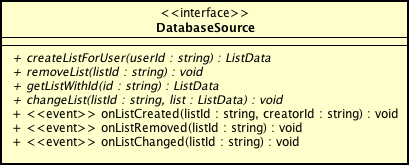
\includegraphics[scale=0.5]{Sezioni/SottosezioniST/img/app/DatabaseSource.png}
	\caption{bringit::server::database::DatabaseSource}
\end{figure}

\begin{itemize}
\item \textbf{Descrizione}: Interfaccia che permette la comunicazione tra il model ed il database sul quale verranno salvati tutti i dati relativi alle varie liste. I metodi da essa esposti non vengono descritti nel dettaglio in quanto l'implementazione di questa interfaccia utilizzerà i noti metodi di Meteor.js, descritti approfonditamente nella rispettiva documentazione inserita all'interno dei riferimenti normativi.
\item \textbf{Utilizzo}: Interfaccia che permette di salvare, modificare, rimuovere dati all'interno del database.
\item \textbf{Attributi}:
	\begin{itemize}
		\item \textit{private listCollection}\\
		La collezione di tutti i messaggi presenti in rocket.chat.
	\end{itemize}
\item \textbf{Metodi}:
	\begin{itemize}
	\item \textit{public DatabaseSource(userId:string):DatabaseSource}\\
	Il costruttore di DatabaseSource.
	 
	\item \textit{public getLists():ListData[]}\\
	Questo metodo ritorna tutte le liste salvate attualmente nel database.
	\item \textit{public removeList(listId:Mongo.ObjectID):void}\\
	Questo metodo rimuove la lista corrispondente all'id passato come parametro dal database.
				\\ \textbf{Parametri}: \begin{itemize}
			\item \textit{listId:Mongo.ObjectID}\\
			L'id della lista che si vuole rimuovere dal database.
			\end{itemize} 
			
	\item \textit{public getListWithId(listId:Mongo.ObjectID):ListData}\\
	Questo metodo ritorna una la lista, recuperata dal database, corrispondente all'id passato come parametro.
				\\ \textbf{Parametri}: \begin{itemize}
			\item \textit{listId:Mongo.ObjectID}\\
			L'id della lista che si vuole recuperare dal database.
			\end{itemize} 
			
	\item \textit{public saveList(listData:ListData):void}\\
	Questo metodo salva la lista data nel database.
				\\ \textbf{Parametri}: \begin{itemize}
			\item \textit{listData:ListData}\\
			La lista che si vuole salvare.
					\end{itemize}
	\item \textit{public getItemWithId(itemId:Mongo.ObjectID):ListItem}\\
	Ritorna il listItem con id corrispondente a quello passato per parametro che è attualmente salvato nel database.
			\\ \textbf{Parametri}: \begin{itemize}
			\item \textit{itemId:Mongo.ObjectID}\\
			L'id del prodotto che si vuole recuperare dal database.
			\end{itemize}
	\item \textit{public clear():void}\\
	Pulisce tutti gli oggetti presenti in tutte le collezioni del database.
	\item \textit{private convertToListData(data:JSONObject):ListData}\\
	Converte un file json opportuno in un oggetto di tipo ListData con gli attributi richiesti.
			\\ \textbf{Parametri}: \begin{itemize}
			\item \textit{data:JSONObject}\\
			Il json che si vuole convertire in ListData.
			\end{itemize}
	\item \textit{private convertToListData(item:JSONObject):ListItem}\\
	Converte un file json opportuno in un oggetto di tipo ListItem con gli attributi richiesti.
			\\ \textbf{Parametri}: \begin{itemize}
			\item \textit{item:JSONObject}\\
			Il json che si vuole convertire in ListItem.
			\end{itemize}
	\end{itemize}
\item \textbf{Eventi}:
\end{itemize}
